\documentclass[11pt,a4paper]{article}
\usepackage[T1]{fontenc}
\usepackage[utf8]{inputenc}
\usepackage{libertinus}
\usepackage{microtype}
\usepackage[margin=27mm,headheight=14pt]{geometry}
\usepackage{amsmath,amssymb,amsthm,mathtools}
\usepackage{libertinust1math}
\usepackage{booktabs,array,graphicx}
\usepackage[table]{xcolor}
\usepackage[most]{tcolorbox}
\usepackage{enumitem}
\usepackage{fancyhdr}
\usepackage{titlesec}
\usepackage{xurl}
\usepackage{hyperref}
\definecolor{ink}{HTML}{18334A}
\definecolor{accent}{HTML}{176B74}
\definecolor{pale}{HTML}{EDF5F6}
\hypersetup{colorlinks=true,linkcolor=accent,citecolor=accent,urlcolor=accent,
 pdftitle={A proof of the Apery Hankel growth conjecture},
 pdfauthor={ChatGPT},pdfsubject={OEIS A228143; exact computations and elementary proofs}}
\titleformat{\section}{\Large\bfseries\color{ink}}{\thesection}{0.65em}{}
\titleformat{\subsection}{\large\bfseries\color{ink}}{\thesubsection}{0.65em}{}
\pagestyle{fancy}\fancyhf{}
\fancyhead[L]{\small\color{ink}Ap\'ery Hankel determinants}
\fancyhead[R]{\small\color{ink}Research note / 18 September 2026}
\fancyfoot[C]{\small\thepage}
\renewcommand{\headrulewidth}{0.3pt}
\setlength{\parskip}{4pt}
\setlength{\parindent}{1.1em}
\setlength{\emergencystretch}{1.5em}
\numberwithin{equation}{section}
\newtheorem{theorem}{Theorem}[section]
\newtheorem{lemma}[theorem]{Lemma}
\newtheorem{corollary}[theorem]{Corollary}
\newtheorem{proposition}[theorem]{Proposition}
\theoremstyle{remark}\newtheorem{remark}[theorem]{Remark}
\newcommand{\A}{\mathsf A}
\newcommand{\J}{\mathcal J}
\newcommand{\dd}{\,\mathrm d}
\newcommand{\R}{\mathbb R}
\newcommand{\N}{\mathbb N}
\newcommand{\abs}[1]{\lvert#1\rvert}
\newcommand{\sourceinput}{\textbf{Known input.}}
\newtcolorbox{resultbox}{colback=pale,colframe=accent,boxrule=0.6pt,
 arc=1.5mm,left=3mm,right=3mm,top=2mm,bottom=2mm}
\title{\vspace{-1.3em}\color{ink}\textbf{A proof of the Ap\'ery Hankel\texorpdfstring{\\}{ }growth conjecture}\vspace{0.25em}\\
\large OEIS A228143, linearly shifted determinants,\texorpdfstring{\\}{ }and a non-D-finite generating series}
\author{Research report prepared with ChatGPT}
\date{18 September 2026}

\begin{document}
\maketitle
\thispagestyle{empty}
\begin{abstract}
For the Ap\'ery numbers $A_k=\sum_{j=0}^k\binom{k}{j}^2\binom{k+j}{j}^2$, let
$D_n=\det(A_{i+j})_{0\leq i,j\leq n}$. The OEIS entry A228143 records a conjecture,
added by Vaclav Kotesovec on 13 September 2026, that
$D_n^{1/n^2}\to(1+\sqrt2)^4/4$. Starting from Edgar's known positive moment-density
theorem, we prove this limit and the stronger estimate
$\log D_n=n(n+1)\log((1+\sqrt2)^4/4)+O(n)$.
The proof uses a polynomial lower bound for the density, monic orthogonal
polynomials, and elementary Legendre--Chebyshev estimates. We also obtain an
explicit growth law for $\det(A_{m(i+j)+r_n})$ when $m$ is fixed and $r_n/n$
converges, including nonzero linear shifts. A further consequence is that the
formal ordinary generating series of $D_n$ is not D-finite. The package includes
exact determinants through $n=200$, independent arithmetic checks, and runnable
Python and C++/GMP code. The density representation is credited, not reproved;
the subsequent determinant arguments are given in full.
\end{abstract}

\begin{resultbox}
\centering
\textbf{Main result}\par\medskip
$\displaystyle
\lim_{n\to\infty}D_n^{1/n^2}
=\frac{17+12\sqrt2}{4}
=8.4926406871192851464\ldots.$\par\medskip
More precisely, some $\kappa>0$ satisfies, for every $n\geq0$,\par\smallskip
$\displaystyle
\kappa^n\left(\frac{17+12\sqrt2}{4}\right)^{n(n+1)}
\leq D_n\leq
4^n\left(\frac{17+12\sqrt2}{4}\right)^{n(n+1)}.$
\end{resultbox}

\noindent\textbf{Status and attribution.}
This is a proof of the precise assertion still labelled a conjecture in the
accessed OEIS revision, not a claim that the result has no antecedent anywhere
in the literature. The essential pre-existing analytic input is G.~A.~Edgar's
work. This report has not been peer reviewed or formalized in a proof assistant.

\newpage
\section{The selected problem and the stronger result}
The Ap\'ery numbers, OEIS A005259, are
\begin{equation}\label{eq:apery}
 A_k=\sum_{j=0}^{k}\binom{k}{j}^{\!2}\binom{k+j}{j}^{\!2},
 \qquad A_0=1,\quad A_1=5,\quad A_2=73.
\end{equation}
Define the leading Hankel determinants
\begin{equation}\label{eq:det}
 D_n=\det\bigl(A_{i+j}\bigr)_{0\leq i,j\leq n}.
\end{equation}
Thus the matrix has order $n+1$, not $n$. The first values are
$1,48,161856,39002646528,\ldots$; they agree with OEIS A228143
\cite{oeis-apery,oeis-hankel}.

The target is the asymptotic formula in the \texttt{\%F} field of revision
\texttt{\#40} of A228143, dated 13 September 2026. It is attributed to Vaclav
Kotesovec and asserts
\begin{equation}\label{eq:conjecture}
 \lim_{n\to\infty}D_n^{1/n^2}=\frac{(1+\sqrt2)^4}{4}.
\end{equation}
It is distinct from the divisibility and root-integrality assertions also
recorded in that entry. The source status here refers to the version accessed
on 18 September 2026 \cite{oeis-hankel}.

Use the constants
\begin{equation}\label{eq:constants}
 C=17+12\sqrt2=(1+\sqrt2)^4,\qquad
 c=C^{-1}=17-12\sqrt2,\qquad \Lambda=\frac C4.
\end{equation}
The small positive number $c$ is an interior singular point of the moment
density; it is \emph{not} the left endpoint of its support.

\begin{theorem}\label{thm:main}
There exists $\kappa\in(0,1]$ such that
\begin{equation}\label{eq:sandwich}
 \kappa^n\Lambda^{n(n+1)}\leq D_n\leq
 4^n\Lambda^{n(n+1)}\qquad(n\geq0).
\end{equation}
Consequently,
\begin{align}
 \log D_n&=n(n+1)\log\Lambda+O(n),\label{eq:logmain}\\
 D_n^{1/n^2}&=\Lambda\exp\bigl(O(1/n)\bigr),\label{eq:rootmain}\\
 \left(\frac{D_n}{D_{n-1}}\right)^{1/(2n)}&\longrightarrow\Lambda
 \qquad(n\to\infty).\label{eq:ratiomain}
\end{align}
In particular, \eqref{eq:conjecture} is true.
\end{theorem}

The proof will bound each monic orthogonal-polynomial norm separately.
This is stronger than trying to estimate one large determinant after replacing
its entries by asymptotic approximations. The latter operation is generally
unsafe; Section~\ref{sec:pitfall} gives an exact counterexample to that method.

\section{The known moment density and a global lower bound}
\label{sec:density}
\sourceinput\quad Edgar's Theorem~1, Proposition~4, Notation~6,
Propositions~25--26, and Corollary~27 \cite{edgar} give an integrable density
$\varphi$ on $[0,C]$ such that
\begin{equation}\label{eq:moments}
 A_k=\int_0^C x^k\varphi(x)\dd x,\qquad \int_0^C\varphi(x)\dd x=1.
\end{equation}
It is positive and real analytic on $(0,c)$ and $(c,C)$, with
\begin{align}
 \varphi(x)&=-\frac6{\pi^2}\log x+o(1) &&(x\downarrow0),\label{eq:left}\\
 \varphi(x)&=\frac{(C-x)^{1/2}}{2^{5/4}C\pi^2}
       +O\bigl((C-x)^{3/2}\bigr) &&(x\uparrow C).\label{eq:right}
\end{align}
At $c$, on each side, it is a nonzero combination of convergent Frobenius
solutions with leading orders $0,\tfrac12,1$. Here our $C,c$ correspond to
Edgar's $c,c_0$.

In particular, for positive distance $t$ from $c$ on either side, the first
nonzero term gives
\begin{equation}\label{eq:interior}
 \varphi(c\pm t)=a_\pm t^{\alpha_\pm}(1+o(1)),\qquad
 a_\pm>0,\quad\alpha_\pm\in\{0,\tfrac12,1\}.
\end{equation}
Indeed, the three basis solutions start with distinct powers. A nonzero
solution has a first nonzero coefficient, and positivity fixes the sign of
its leading term. No value of $\varphi(c)$ needs to be assigned, and equality
of its one-sided limits is not required below.

\begin{lemma}[Polynomial minorant]\label{lem:minorant}
Let $Q(x)=(x-c)(x-C)$. There is $\eta>0$ such that
\begin{equation}\label{eq:minorant}
 \varphi(x)\geq\eta Q(x)^2
 \quad\text{for almost every }x\in[0,C].
\end{equation}
\end{lemma}
\begin{proof}
Consider $R(x)=\varphi(x)/Q(x)^2$ away from $c,C$.
On each of $(0,c)$ and $(c,C)$ this is continuous and positive.
Since $cC=1$, $Q(0)=1$, and \eqref{eq:left} implies $R(x)\to+\infty$
as $x\downarrow0$. Equation~\eqref{eq:right} gives
$R(x)\asymp(C-x)^{-3/2}\to+\infty$ as $x\uparrow C$.
At $c$, \eqref{eq:interior} gives
$R(c\pm t)\asymp t^{\alpha_\pm-2}\to+\infty$.
Choose small neighborhoods of these three points on which $R$ is bounded
below by a positive constant. On the remaining compact pieces, its positive
continuous minimum is also positive. The least of these bounds is an
admissible $\eta$.
\end{proof}

The interior singularity is the delicate point in this argument. Positivity
alone would not justify a strictly positive uniform lower bound for the
density. Squaring a polynomial that vanishes at $c$ and $C$ avoids that
incorrect inference. The constant $\eta$ is established to exist; this report
does not claim a certified numerical value for it.

\section{Elementary norm estimates and the proof}
\subsection{A moment determinant is a product of minimum norms}
For a nonzero real polynomial $p$, positivity of $\varphi$ on an interval gives
$\int p(x)^2\varphi(x)\dd x>0$. Thus its polynomial inner product is positive
definite. Let $p_k$ be its monic orthogonal polynomial of degree $k$, and put
\begin{equation}\label{eq:hk}
 h_k=\int_0^C p_k(x)^2\varphi(x)\dd x
 =\min_{\substack{p\in\R[x]\text{ monic}\\\deg p=k}}
      \int_0^C p(x)^2\varphi(x)\dd x.
\end{equation}
The minimum follows by writing $p=p_k+q$, $\deg q<k$, and using orthogonality.
The change of basis from $1,x,\ldots,x^n$ to $p_0,\ldots,p_n$ is unitriangular.
Its determinant is one, so taking Gram determinants gives
\begin{equation}\label{eq:product}
 D_n=\prod_{k=0}^n h_k,\qquad h_0=1.
\end{equation}
These are the usual monic-norm identities; compare DLMF \S18.2
\cite{dlmf}. The argument above also proves $D_n>0$ for every $n$.

\subsection{The Lebesgue lower comparison}
\begin{lemma}\label{lem:legendre}
For $L>0$ and $k\geq0$, the minimum squared norm of a monic polynomial of
degree $k$ for Lebesgue measure on $[0,L]$ is
\begin{equation}\label{eq:legendre}
 \ell_k(0;L)=\frac{L^{2k+1}}{(2k+1)\binom{2k}{k}^2}
 \geq L\left(\frac L4\right)^{2k}.
\end{equation}
\end{lemma}
\begin{proof}
On $[0,1]$, the polynomial
\[
 R_k(t)=\frac1{k!}\frac{\mathrm d^k}{\mathrm dt^k}
       \bigl[t^k(t-1)^k\bigr]
\]
is orthogonal to all lower-degree polynomials by $k$ integrations by parts.
Its leading coefficient is $\binom{2k}{k}$. Another integration by parts gives
\[
 \int_0^1 R_k(t)t^k\dd t
 =\int_0^1 t^k(1-t)^k\dd t
 =\frac{(k!)^2}{(2k+1)!}.
\]
Orthogonality therefore implies $\int_0^1R_k(t)^2\dd t=1/(2k+1)$.
Dividing by its leading coefficient and scaling $x=Lt$ proves the equality
in \eqref{eq:legendre} and the minimizing property.

For the inequality, set $u_k=(2k+1)\binom{2k}{k}^2/16^k$. Direct cancellation
gives $u_0=1$ and
\[
 \frac{u_{k+1}}{u_k}=1-\frac1{4(k+1)^2}<1.
\]
Thus $(2k+1)\binom{2k}{k}^2\leq16^k$, as needed.
\end{proof}

If $p$ is monic of degree $k$, then $pQ$ is monic of degree $k+2$.
Lemmas~\ref{lem:minorant} and \ref{lem:legendre} give
\[
 \int_0^C p(x)^2\varphi(x)\dd x
 \geq\eta\int_0^C(p(x)Q(x))^2\dd x
 \geq\eta\ell_{k+2}(0;C)
 \geq\eta C\Lambda^{2k+4}.
\]
Consequently, with
\begin{equation}\label{eq:kappa}
 \kappa=\eta C\Lambda^4>0,
 \qquad h_k\geq\kappa\Lambda^{2k}\quad(k\geq0).
\end{equation}
The case $k=0$, together with $h_0=1$, shows $\kappa\leq1$.

\subsection{The Chebyshev upper comparison}
The Chebyshev polynomial $T_k$ satisfies $T_k(\cos\theta)=\cos(k\theta)$.
The recurrence $T_{k+1}(t)=2tT_k(t)-T_{k-1}(t)$ shows that its leading
coefficient is $2^{k-1}$ for $k\geq1$. Hence
\[
 q_k(x)=2\Lambda^k T_k\left(\frac{2x}{C}-1\right)
\]
is monic of degree $k$ and has absolute value at most $2\Lambda^k$ on $[0,C]$.
Since the measure has total mass one, the minimum in \eqref{eq:hk} satisfies
\begin{equation}\label{eq:uppernorm}
 h_k\leq\int_0^Cq_k(x)^2\varphi(x)\dd x\leq4\Lambda^{2k}
 \qquad(k\geq1).
\end{equation}

\begin{proof}[Proof of Theorem~\ref{thm:main}]
Multiply \eqref{eq:kappa} and \eqref{eq:uppernorm} over $k=1,\ldots,n$ and
use \eqref{eq:product} with $h_0=1$. Since $2\sum_{k=1}^n k=n(n+1)$, this
is \eqref{eq:sandwich}. Taking logarithms gives \eqref{eq:logmain}; dividing
by $n^2$ gives \eqref{eq:rootmain}. Finally $D_n/D_{n-1}=h_n$, and the
individual bounds imply
\[
 \Lambda\kappa^{1/(2n)}\leq h_n^{1/(2n)}\leq\Lambda4^{1/(2n)},
\]
which proves \eqref{eq:ratiomain}.
\end{proof}

\begin{remark}
The proof does not assert that $h_n/\Lambda^{2n}$ converges. It proves this
sequence is bounded above and bounded away from zero. Nor does
\eqref{eq:logmain} give a full multiplicative asymptotic equivalent for $D_n$.
\end{remark}

\section{An explicit law for linearly shifted determinants}
\label{sec:shifts}
The same comparison idea gives more than fixed shifts. For integers $m\geq1$
and $r\geq0$, define
\begin{equation}\label{eq:shiftdef}
 H_n^{(m,r)}=\det\bigl(A_{m(i+j)+r}\bigr)_{0\leq i,j\leq n}.
\end{equation}
Here $m$ is the stride in the moment indices. The shift $r$ is held constant
throughout each matrix, but may vary from one matrix size to another.

Define, for $\sigma\geq0$,
\begin{equation}\label{eq:Psi}
 \Psi(\sigma)=\frac12\left[
 (\sigma+2)^2\log(\sigma+2)-2(\sigma+1)^2\log(\sigma+1)
 +\sigma^2\log\sigma\right],
\end{equation}
with $0^2\log0:=0$.

\begin{theorem}[Linear-shift growth law]\label{thm:shift}
Fix a positive integer $m$. If $r_n$ are nonnegative integers and
$r_n/n\to\rho\in[0,\infty)$, then
\begin{equation}\label{eq:shiftlaw}
 \lim_{n\to\infty}\frac{\log H_n^{(m,r_n)}}{n^2}
 =(m+\rho)\log C-\Psi(\rho/m).
\end{equation}
Equivalently,
\[
 \lim_{n\to\infty}\bigl(H_n^{(m,r_n)}\bigr)^{1/n^2}
 =C^{m+\rho}\exp\bigl(-\Psi(\rho/m)\bigr).
\]
In particular, every sublinear shift $r_n=o(n)$ has limit $C^m/4$.
\end{theorem}

For example,
\begin{align}
 \lim_{n\to\infty}\det(A_{2i+2j})_{0\leq i,j\leq n}^{1/n^2}
   &=\frac{C^2}{4},\label{eq:stride2}\\
 \lim_{n\to\infty}\det(A_{i+j+n})_{0\leq i,j\leq n}^{1/n^2}
   &=\frac{16C^2}{81\sqrt3}.\label{eq:linear1}
\end{align}
The constant $C^m/4$ for a stride $m$ is not $(C/4)^m$. The proof below also
provides a finite-size comparison with a completely explicit determinant.

\subsection{The power-weight model}
For $s>-1$ and $L>0$, put
\begin{equation}\label{eq:Jdef}
 \J_n(s;L)=\det\left(\frac{L^{i+j+s+1}}{i+j+s+1}\right)_{0\leq i,j\leq n}.
\end{equation}
This is the moment determinant of $y^s\dd y$ on $[0,L]$.
Its monic minimum norms are
\begin{equation}\label{eq:jacobinorm}
 \ell_k(s;L)=\frac{L^{2k+s+1}}
 {(2k+s+1)\binom{2k+s}{k}^2},\qquad
 \binom{2k+s}{k}=\prod_{j=1}^k\frac{k+s+j}{j}.
\end{equation}
To verify \eqref{eq:jacobinorm}, replace the Rodrigues polynomial in
Lemma~\ref{lem:legendre} by
\[
 R_{k,s}(t)=\frac{t^{-s}}{k!}\frac{\mathrm d^k}{\mathrm dt^k}
        \bigl[t^{k+s}(t-1)^k\bigr].
\]
It is a polynomial of degree $k$, with leading coefficient
$\binom{2k+s}{k}$. Integration by parts proves orthogonality for weight $t^s$.
The boundary terms vanish because $s>-1$. Its pairing with $t^k$ is the beta
integral $\int_0^1t^{k+s}(1-t)^k\dd t$; dividing by the leading coefficient
and scaling the interval gives \eqref{eq:jacobinorm}.

We will use both its norm product and its Cauchy determinant form:
\begin{equation}\label{eq:Jexact}
 \J_n(s;L)=\prod_{k=0}^n\ell_k(s;L)
 =L^{(n+1)(n+s+1)}
   \frac{\prod_{j=0}^n(j!)^2}
        {\prod_{i=0}^n\prod_{j=0}^n(s+1+i+j)}.
\end{equation}
For completeness, the second equality follows by factoring powers of $L$
and applying the Cauchy identity
\[
 \det\left(\frac1{x_i+y_j}\right)
 =\frac{\prod_{i<j}(x_j-x_i)(y_j-y_i)}{\prod_{i,j}(x_i+y_j)}
\]
with $x_i=i$, $y_j=s+1+j$. One elementary proof of that identity clears the
common denominator: the resulting polynomial is alternating in the $x_i$
and in the $y_j$, so is divisible by both Vandermonde products. Total degrees
agree. The remaining constant is one, by induction on the residue at
$x_n=-y_n$, starting with the $1\times1$ case.

\subsection{Uniform comparison with the power-weight model}
\begin{proposition}\label{prop:comparison}
For fixed $m\geq1$ and $T<\infty$, uniformly for integers $0\leq r\leq Tn$,
\begin{equation}\label{eq:modelcomparison}
 \log H_n^{(m,r)}=\log\J_n(r/m;C^m)+O_{m,T}(n)
 \qquad(n\geq1).
\end{equation}
\end{proposition}
\begin{proof}
Set $L=C^m$, $a=c^m$, $s=r/m$, and change variables $y=x^m$ in
\eqref{eq:moments}. The moments in \eqref{eq:shiftdef} are those of
$y^s w_m(y)\dd y$, where
\begin{equation}\label{eq:pushforward}
 w_m(y)=\frac1m y^{1/m-1}\varphi(y^{1/m}),\qquad0<y<L.
\end{equation}
The map is smooth with nonzero derivative near $a$ and $L$. Thus the
one-sided finite orders at $a$ and the square-root order at $L$ are unchanged.
At zero,
\[
 w_m(y)\sim\frac6{m^2\pi^2}y^{1/m-1}\log(1/y)\longrightarrow+\infty.
\]
The argument of Lemma~\ref{lem:minorant} therefore supplies $\eta_m>0$ with
$w_m(y)\geq\eta_m[(y-a)(y-L)]^2$ almost everywhere.

Set $\beta=-1+1/(2m)\in(-1,0)$. Near zero,
$w_m(y)/y^\beta\to0$, and this ratio is bounded on the remaining intervals,
including their one-sided limits at $a$ and $L$. Hence a constant $K_m>0$
also exists such that
\begin{equation}\label{eq:twoenvelopes}
 \eta_m[(y-a)(y-L)]^2\leq w_m(y)\leq K_m y^\beta.
\end{equation}
Neither constant depends on $r$ or $n$.

Let $h_k(s)$ denote the monic minimum norm for $y^s w_m(y)\dd y$.
Multiplication by the monic quadratic on the left of
\eqref{eq:twoenvelopes}, and a minimizing trial polynomial for the upper
power weight, give
\[
 \eta_m\ell_{k+2}(s;L)\leq h_k(s)\leq K_m\ell_k(s+\beta;L).
\]
The parameter $s+\beta$ is greater than $-1$. Multiplying over $k=0,\ldots,n$
yields
\begin{equation}\label{eq:modelbounds}
 \eta_m^{n+1}\J_n(s;L)
 \frac{\ell_{n+1}(s;L)\ell_{n+2}(s;L)}{\ell_0(s;L)\ell_1(s;L)}
 \leq H_n^{(m,r)}\leq K_m^{n+1}\J_n(s+\beta;L).
\end{equation}

We check that both corrections to $\log\J_n(s;L)$ are $O(n)$.
Write $b=-\beta\in(0,1)$. Formula~\eqref{eq:Jexact} gives
\begin{align*}
 \log\frac{\J_n(s+\beta;L)}{\J_n(s;L)}
 &=(n+1)\beta\log L
  -\sum_{i,j=0}^n\log\left(1-\frac b{s+1+i+j}\right).
\end{align*}
For $t\geq1$,
$0\leq-\log(1-b/t)\leq b/((1-b)t)$. Counting pairs with fixed $i+j$ gives
\[
 \sum_{i,j=0}^n\frac1{s+1+i+j}
 \leq\sum_{i,j=0}^n\frac1{1+i+j}\leq2n+1.
\]
Thus the logarithmic upper correction is $O_m(n)$, uniformly in $s\geq0$.

For the lower correction, $s\leq(T/m)n$. At $k=0,1,n+1,n+2$, formula
\eqref{eq:jacobinorm} shows $\abs{\log\ell_k(s;L)}=O_{m,T}(n)$.
For $k=0,1$ this is immediate. For the other two indices use
\[
 1\leq\binom{2k+s}{k}
 \leq\frac{(2k+s)^k}{k!}
 \leq\left(\frac{e(2k+s)}k\right)^k,
\]
whose logarithm is $O_{m,T}(n)$ since $k\geq n+1$ and $s=O(n)$.
Here $k!\geq(k/e)^k$ follows by integrating $\log x$ on $[1,k]$.
The remaining factors in \eqref{eq:jacobinorm} have logarithms $O(n)$ as well.
Applying these estimates to \eqref{eq:modelbounds} proves
\eqref{eq:modelcomparison}.
\end{proof}

\subsection{Evaluating the limiting constant}
\begin{lemma}\label{lem:modelasym}
If $s_n\geq0$ and $s_n/n\to\sigma\geq0$, then
\begin{equation}\label{eq:modelasym}
 \frac1{n^2}\log\J_n(s_n;L)
 \longrightarrow(1+\sigma)\log L-\Psi(\sigma).
\end{equation}
\end{lemma}
\begin{proof}
Taking logarithms in \eqref{eq:Jexact}, the factorial part satisfies
\begin{equation}\label{eq:factorialasym}
 2\sum_{j=0}^n\log(j!)=n^2\log n-\frac32n^2+O(n\log(n+1)).
\end{equation}
For example, interchange the sums to obtain
$2\sum_{k=1}^n(n+1-k)\log k$ and compare the sums of $\log k$ and $k\log k$
with their integrals.
For the denominator, Riemann sums give
\begin{equation}\label{eq:denomasym}
 \frac1{n^2}\sum_{i,j=0}^n\log(s_n+1+i+j)-\log n
 \longrightarrow\int_0^1\!\int_0^1\log(\sigma+x+y)\dd x\dd y.
\end{equation}
When $\sigma>0$ the integrand is continuous. When $\sigma=0$, split off
$i+j\leq\delta n$. The normalized absolute contribution there is bounded by
$O(\delta^2(1+\abs{\log\delta}))+o(1)$: count the $i+j=k$ pairs and use
$\log(n/(k+1))$ as an upper bound for the absolute logarithm for large $n$.
Outside this corner, convergence is uniform. Letting $\delta\downarrow0$
justifies \eqref{eq:denomasym} also at $\sigma=0$.

Two integrations, with $t^2\log t$ assigned its continuous value at zero,
yield
\[
 \int_0^1\!\int_0^1\log(\sigma+x+y)\dd x\dd y
 =\Psi(\sigma)-\frac32.
\]
The two $\tfrac32$ terms cancel between this expression and
\eqref{eq:factorialasym}. The power of $L$ in \eqref{eq:Jexact} contributes
$(1+\sigma)\log L$, proving the claim.
\end{proof}

\begin{proof}[Proof of Theorem~\ref{thm:shift}]
The convergence $r_n/n\to\rho$ implies $r_n\leq Tn$ eventually for some
finite $T$. Apply Proposition~\ref{prop:comparison}, then
Lemma~\ref{lem:modelasym} with $s_n=r_n/m$, $L=C^m$, and
$\sigma=\rho/m$. The error $O(n)$ disappears after division by $n^2$.
Finally $\Psi(0)=\log4$.
\end{proof}

For fixed $m,r$, \eqref{eq:modelcomparison} and the norm formula also give
$\log H_n^{(m,r)}=n(n+1)\log(C^m/4)+O_{m,r}(n)$.
To see this without a further asymptotic theorem, changing the power parameter
from $0$ to a fixed $s=r/m$ changes $\log\J_n$ by $O_s(n)$, using
$\log(1+s/t)\leq s/t$ and the same reciprocal sum estimate as above.
Lemma~\ref{lem:legendre} and the Chebyshev upper comparison for Lebesgue
measure then bound $\log\J_n(0;L)-n(n+1)\log(L/4)$ by $O_L(n)$.
The stride $m$ is fixed throughout these statements; no uniform assertion for
$m\to\infty$ is made.

\section{A generating-function consequence}
\label{sec:dfinite}
\begin{theorem}\label{thm:nonrecursive}
The sequence $(D_n)$ is not P-recursive over $\mathbb C$. Its formal ordinary
generating series $F(z)=\sum_{n\geq0}D_nz^n$ is not D-finite.
Moreover, for every fixed real $s$, the series
$\sum_{n\geq0}D_n z^n/(n!)^s$ has radius of convergence zero.
\end{theorem}
\begin{proof}
Suppose that, for all sufficiently large integers $n$,
\begin{equation}\label{eq:prec}
 \sum_{j=0}^q P_j(n)D_{n+j}=0,
 \qquad P_j\in\mathbb C[n],\quad P_q\not\equiv0.
\end{equation}
The case $q=0$ contradicts $D_n>0$. For $q\geq1$, the leading coefficient
polynomial has no zeros at sufficiently large integers. Ratios of the other
coefficient polynomials to it have at most polynomial growth. Therefore
some $K>0$, integer $d\geq0$, and $N$ satisfy
\[
 \abs{D_{n+q}}\leq K n^d\max_{0\leq j<q}\abs{D_{n+j}}\qquad(n\geq N).
\]
Taking running maxima and increasing $K$ if necessary gives
$\abs{D_n}\leq K_0K_1^n(n!)^d$. Thus
$\log D_n=O(n\log n)$, contradicting \eqref{eq:logmain}, since $\Lambda>1$.
This proves the first assertion.

A polynomial-coefficient linear differential equation for $F$ would, by
coefficient comparison, give a nontrivial polynomial-coefficient recurrence
for its coefficients for all sufficiently large indices. Hence $F$ cannot
be D-finite. This argument is about formal power series and does not assume
that $F$ converges.

Finally,
\[
 \frac1n\log\frac{D_n}{(n!)^s}
 =n\log\Lambda+O(\log(n+1))\longrightarrow+\infty.
\]
The root test gives radius zero for every fixed $s$.
\end{proof}

Divergence alone would \emph{not} have proved non-D-finiteness: a formal
D-finite series can have radius zero. The polynomial-recurrence growth bound
is the essential extra argument.

\section{Why entrywise asymptotics do not determine this limit}
\label{sec:pitfall}
Consider, for $0\leq a<C$, the elementary moments
\[
 m_k^{(a)}=\int_a^Cx^k\dd x=\frac{C^{k+1}-a^{k+1}}{k+1}.
\]
For each fixed $0<a<C$,
\[
 \frac{m_k^{(a)}}{m_k^{(0)}}=1-(a/C)^{k+1}.
\]
Thus these two moment sequences agree to every algebraic relative asymptotic
order in $1/k$, with an exponentially small relative difference.
Nevertheless their determinant limits differ.
Translation by $a$ is a unitriangular change of the monomial basis, so it does
not change a Gram determinant. Applying Lemma~\ref{lem:legendre} on the
translated interval of length $C-a$ gives the exact formula
\begin{equation}\label{eq:counterexample}
 \det(m_{i+j}^{(a)})_{0\leq i,j\leq n}
 =\frac{(C-a)^{(n+1)^2}}
 {\prod_{k=0}^n(2k+1)\binom{2k}{k}^2}.
\end{equation}
Its $n^2$-root limit is $(C-a)/4$, rather than $C/4$.
Indeed, the same lower and upper monic-norm comparisons used above prove
this limit directly.

This is a counterexample to a tempting inference about Hankel determinants,
not to Kotesovec's conjecture. It explains why a single-entry asymptotic
formula cannot safely be substituted into a growing determinant. In the
Ap\'ery case, incorrectly discarding the short interval $(0,c)$ would likewise
suggest the wrong constant
\[
 \frac{C-c}{4}=6\sqrt2=8.485281374\ldots,
 \qquad\text{instead of}\qquad
 \frac C4=8.492640687\ldots.
\]
The full positive support and the global comparison in
Lemma~\ref{lem:minorant} retain this small but consequential interval.

\section{Exact computations and independent checks}
\label{sec:computations}
The calculations supplement, but are not used as premises of, the proof.
Moments were generated using the classical recurrence
\begin{equation}\label{eq:recurrence}
 (k+1)^3A_{k+1}
 =(2k+1)(17k^2+17k+5)A_k-k^3A_{k-1},
 \qquad A_0=1,\ A_1=5,
\end{equation}
recorded in Edgar's equation~(1) and OEIS A005259 \cite{edgar,oeis-apery}.
A symmetric fraction-free elimination pass on the $201\times201$ Hankel
matrix produced $D_0,\ldots,D_{200}$ as exact integers.
At pivot $k$, the update was
\begin{equation}\label{eq:bareiss}
 a_{ij}^{\mathrm{new}}
 =\frac{a_{kk}a_{ij}-a_{ik}a_{kj}}{p},\qquad i,j>k,
\end{equation}
where $p$ is the preceding pivot, initially $1$. Every division was checked
for zero remainder. Positivity of all leading minors means no pivoting is
needed in this application. Successive pivots give the successive leading
determinants. There were exactly $200\cdot201\cdot202/6=1{,}353{,}400$
checked divisions in the symmetric update; $D_{200}$ has $37{,}308$ decimal
digits. The recorded GMP determinant phase took about $124$ seconds in this
runtime, a measurement rather than a performance guarantee.

\begin{table}[htbp]
\centering
\small
\begin{tabular}{p{0.75\linewidth}rr}
\toprule
Check & Count & Result \\
\midrule
Recurrence vs. defining binomial sum ($0\leq k\leq400$) & 401 & Pass \\
Displayed OEIS prefix ($D_0,\ldots,D_9$) & 10 & Pass \\
Python vs. GMP ($D_0,\ldots,D_{40}$) & 41 & Pass \\
Independent rational Gaussian determinants ($n\leq12$) & 13 & Pass \\
Independent modular determinants (11 sizes, 3 primes) & 33 & Pass \\
Shifted Desnanot--Jacobi identities & 64 & Pass \\
Power-weight Cauchy determinants, rational parameters & 32 & Pass \\
Central-binomial inequality ($0\leq k\leq500$) & 501 & Pass \\
\bottomrule
\end{tabular}
\caption{Exact verification results. The full integer divisions were also checked during generation.}\label{tab:verification}
\end{table}


\begin{samepage}
Table~\ref{tab:numerical} and Figure~\ref{fig:convergence} use logarithms of
these exact integers, not floating-point determinants. Hankel determinant
formulas are known to be ill-conditioned in direct numerical use; DLMF
\S18.2(ix) explicitly warns about this issue \cite{dlmf}.
The displayed decimal values are numerical evaluations, not interval-certified
bounds. The exact data and exact-arithmetic checks are provided separately.\par
\end{samepage}

\begin{table}[htbp]
\centering
\small
\begin{tabular}{rrr}
\toprule
$n$ & $D_n^{1/n^2}$ & $(D_n/D_{n-1})^{1/(2n)}$ \\
\midrule
1 & 48.0000000000 & 6.9282032303 \\
2 & 20.0577493937 & 7.6202968816 \\
5 & 11.9387651922 & 8.1187083186 \\
10 & 10.0601045949 & 8.3009844581 \\
20 & 9.2400493095 & 8.3954447392 \\
50 & 8.7832622606 & 8.4538328708 \\
100 & 8.6366837149 & 8.4732336106 \\
200 & 8.5643598268 & 8.4829390793 \\
\bottomrule
\end{tabular}
\caption{Root diagnostics computed from exact integers; the common limit is $\Lambda=8.492640687119\ldots$.}\label{tab:numerical}
\end{table}


\begin{figure}[htbp]
 \centering
 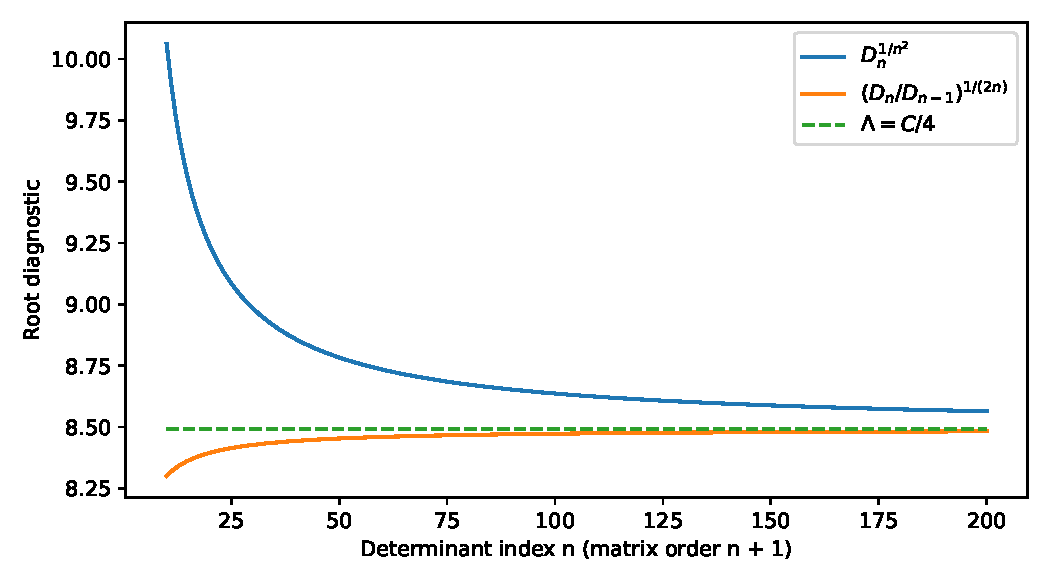
\includegraphics[width=0.96\linewidth]{figures/convergence.pdf}
 \caption{Two root diagnostics from exact determinants, for $10\leq n\leq200$.
 The horizontal line is the proved limit $\Lambda$. The finite-sample placement
 of the curves above or below it is an observation, not a claim of monotonicity
 or a separate theorem.}\label{fig:convergence}
\end{figure}

The shift experiment file records exact samples at $n=10,20,40,80$.
The three families have $(m,r_n)=(1,n)$, $(2,0)$, and $(2,n)$. For each sample the shift is fixed throughout
that matrix. Samples through $n=20$ were also computed with the Python
implementation. Their numerical roots, compared to the limits in
Theorem~\ref{thm:shift}, appear in Table~\ref{tab:shifts}.
\begin{table}[htbp]
\centering
\small
\begin{tabular}{rrrrr}
\toprule
$(m,\rho)$ & Proved limit & $n=20$ & $n=40$ & $n=80$ \\
\midrule
$(1,1)$ & 131.6072514 & 154.1754400 & 142.5207807 & 136.9744192 \\
$(2,0)$ & 288.4997834 & 360.3947981 & 322.3570941 & 304.9315450 \\
$(2,1)$ & 6075.4685812 & 8406.8961687 & 7151.9818542 & 6593.0434765 \\
\bottomrule
\end{tabular}
\caption{Numerical values of $(H_n^{(m,r_n)})^{1/n^2}$ for $r_n=\rho n$. The limits follow from the theorem, not from extrapolation.}\label{tab:shifts}
\end{table}


\section{What has and has not been established}
The established conclusion is a proof of the stated OEIS growth limit, using
a previously known positive density theorem, with a stronger $O(n)$ error
in the logarithm. The same method yields the explicit linear-shift law and
the non-D-finiteness corollary. In particular, the work is not only a search
for a numerical counterexample: the target conjecture turns out to admit a
positive proof.

The analysis does not evaluate the best lower-envelope constant $\eta$,
determine a limit for $h_n/\Lambda^{2n}$, or give a full multiplicative
asymptotic equivalent such as $D_n\sim K\Lambda^{n^2}B^n n^\gamma$.
None of the other arithmetic assertions on A228143 is being claimed here as
a newly solved problem. The literature check establishes the status of the
specific accessed entry, not worldwide priority for every consequence of
Edgar's theorem.

A natural continuation is to determine the finer normalized norm and
determinant asymptotics while treating the interior singular point and the
logarithmic endpoint accurately. The elementary comparisons already settle
the leading growth questions; finer constants require additional arguments,
not extrapolation from the data.

\appendix
\section{Reproducing and auditing the package}
The supplied files have separate roles. The article contains the proof.
The file \path{data/determinants_0_200.txt} is not distributed with the
archive; \path{build/apery_gmp 200} rebuilds it. It contains exact integers;
\texttt{code/apery\_exact.py} is a standard-library Python implementation;
\texttt{code/apery\_gmp.cpp} is the faster C++17/GMP implementation;
and \texttt{code/verify.py} performs the independent arithmetic checks.
The plotting script additionally uses \texttt{mpmath} and \texttt{matplotlib}.
The saved verification log records the actual checks performed.

From the package directory, the exact checks can be rerun with
\begin{quote}\small\ttfamily
python3 code/verify.py
\end{quote}
A smaller exact table can be regenerated without external Python packages:
\begin{quote}\small\ttfamily
python3 code/apery\_exact.py --n 40 --output data/recomputed.txt
\end{quote}
For the full table, compile the supplied GMP implementation and run it with
argument \texttt{200}; the complete commands are in \texttt{README.md}.
That program reports a failure rather than silently accepting a nonexact
division or nonpositive pivot. \texttt{shift\_experiments.py} similarly runs
shifted examples and can use either implementation.

The symmetric elimination uses $O(n^3)$ integer arithmetic operations and
$O(n^2)$ integer storage locations. These are \emph{not} bit-complexity bounds:
the integers grow with the determinant size. No claim of a faster asymptotic
determinant algorithm is made. The PDF was compiled from this source and
rendered for layout inspection. There is no Lean proof or external OEIS
submission in the package.

\begin{thebibliography}{9}
\bibitem{oeis-hankel}
The OEIS Foundation Inc., \emph{A228143: Hankel-type determinants of the
Ap\'ery numbers}. Sequence by Zhi-Wei Sun; growth conjecture attributed to
Vaclav Kotesovec, 13 September 2026. Internal revision \texttt{\#40},
13 September 2026, accessed 18 September 2026.
\url{https://oeis.org/A228143/internal}.

\bibitem{oeis-apery}
The OEIS Foundation Inc., \emph{A005259: Ap\'ery numbers}.
Accessed 18 September 2026.
\url{https://oeis.org/A005259}.

\bibitem{edgar}
G.~A.~Edgar, \emph{The Ap\'ery Numbers as a Stieltjes Moment Sequence},
arXiv:2005.10733v2, 2 September 2020.
Theorem~1, Proposition~4, Notation~6, Propositions~25--26, Corollary~27,
and equation~(1).
\url{https://arxiv.org/abs/2005.10733}.

\bibitem{dlmf}
NIST Digital Library of Mathematical Functions, \S18.2,
\emph{General Orthogonal Polynomials}, especially the monic norm and Hankel
determinant identities and the numerical-conditioning caution in \S18.2(ix).
Accessed 18 September 2026.
\url{https://dlmf.nist.gov/18.2}.
\end{thebibliography}
\end{document}
